\section{Nowcasting: MIDAS regression}
\label{chapter3_section2}


Another approach to mixed frequency modelling and nowcasting is the MIDAS regression (for MIxed DAta Sampling). This methodology was originally proposed by \cite{Ghysels2004}, with an essentially theoretical approach. More applied aspects of the methodology have then been studied in contributions such as \cite{Ghysels2007} and \cite{Ghysels2009}.


\subsection{Formulation}
\label{chapter3_section2_subsection1}

Similarly to the dynamic factor model, consider the case where one wants to predict one low-frequency variable (say a quarterly variable for instance) by the way of $n$ higher frequency variables (say for instance monthly features). Denote by $t$ the low frequency periods, and assume that the high frequency variables are observed $m$ times during one period of low frequency (so for instance for a quaterly/monthly model, $t$ corresponds to quarters, and there are $m=3$ months between any two quarters). Denote by $y$ the low frequency variable and by $x_{1}, \cdots, x_{n}$ the set of $n$ high frequency features. Because there are $m$ times more periods in the high frequency features, the observation $y_t$ corresponds to the feature observations $x_{1,tm}, \cdots, x_{n,tm}$. The low frequency variable is assumed to be explained by $p$ of its own (low frequency) lags, as well as $q$ (high frequency) lags of the $n$ features.

A simple MIDAS regression can then be formulated as:

\begin{equation}
y_t = \mu + \sum_{j=1}^{p} \gamma_i \ y_{t-j} + \sum_{i=1}^{n} \sum_{j=1}^{q} \beta_{ij} \  x_{i,tm+1-j} + \varepsilon_t \hspace{2cm}
\varepsilon_t \sim N(0, \sigma^2)
\label{equation_c3_s2_ss1_1}
\end{equation}

$\mu$ is an intercept term, $\gamma_i$ are lag-specific coefficients for the low-frequency variable, while $\beta_{ij}$ are feature and lag-specific coefficients. A direct approach would consist in estimating \ref{equation_c3_s2_ss1_1} as it is. However, this strategy might be problematic as one would be quickly facing the curse of dimensionality. Consider for instance the extreme case where $y_t$ is yearly while each $x_{i,t}$ is daily. Assuming 22 open days a month or 264 open days a year, one would have to estimate 264 coefficients $\beta_{ij}$ for each of the $n$ feature to match just one period of the low frequency variable.

\newpage

For this reason, \cite{Ghysels2007} suggest a more parsimonious approach that drastically reduces the dimensionality of the regression. To do so, reformulate \ref{equation_c3_s2_ss1_1} slightly to obtain:

\begin{equation}
y_t = \mu + \sum_{j=1}^{p} \gamma_i \ y_{t-j} + \sum_{i=1}^{n} \beta_i \big( \sum_{j=1}^{q}  w_{ij} \  x_{i,tm+1-j} \big) + \varepsilon_t \hspace{2cm}
\varepsilon_t \sim N(0, \sigma^2)
\label{equation_c3_s2_ss1_2}
\end{equation}

The $\beta_i$ are now purely feature-specific coefficients, while the $w_{i,j}$ are weights such that $\ssumm{j=0}{q} w_{i,j} = 1$ (a requirement for $\beta_i$ to be uniquely defined). The strategy then consists in estimating the numerous weights $w_{i,j}$ for each feature through a small number $k$ of parameters $\theta_i = ( \theta_{i1}, \cdots, \theta_{ik})$. In particular, \cite{Ghysels2007} propose two strategies to estimate the series of $w_{i,j}$ coefficients. The first one relies on the so-called exponential Almon lag polynomial, which for $k=2$ is defined as:

\begin{equation}
w_{ij}(\theta_i) = \frac{\exp(\theta_{i1} j + \theta_{i2} j^2)}{\ssumm{j=1}{q} \exp(\theta_{i,1} j + \theta_{i,2} j^2)}
\label{equation_c3_s2_ss1_3}
\end{equation}

The second approach is the Beta lag approach. It also uses only $k=2$ parameters, and is defined as:

\begin{equation}
w_{ij}(\theta_i) = \frac{x_j^{\theta_{i1}-1} \ (1-x_j)^{\theta_{i2}-1}}{\ssumm{j=1}{q} \ x_j^{\theta_{i1}-1} \ (1-x_j)^{\theta_{i2}-1}} 
\hspace{15mm}
x_j = \frac{j}{q}
\label{equation_c3_s2_ss1_4}
\end{equation}

Both formulations are quite flexible and can handle a wide variety of structures for the weights $w_{i,j}$ (this is discussed in more details in section \ref{chapter3_section2_subsection2}). Once the weights are estimated, there exists a direct correspondance between \ref{equation_c3_s2_ss1_1} and \ref{equation_c3_s2_ss1_2}, the latter implying $\beta_{ij} = \beta_{i} w_{ij}$ in the former. Simply, the estimation of \ref{equation_c3_s2_ss1_2} is considerably more parsimonious, which makes it quite appealing. 



\subsection{Estimation}
\label{chapter3_section2_subsection2}


Estimation of a MIDAS model consists in calculating the values of $\mu, \gamma_i, \beta_i$, and $\theta_i$. Formally, it consists in finding the parameter values that minimize the sum of squared residuals in \ref{equation_c3_s2_ss1_2}:

\begin{equation}
\{ \hat{\mu}, \hat{\gamma}_i, \hat{\beta}_i, \hat{\theta}_i\} = \underset{\mu, \gamma_i, \beta_i, \theta_i}{argmin} 
\left( y_t - \mu - \sum_{j=1}^{p} \gamma_i \ y_{t-j} - \sum_{i=1}^{n} \beta_i \big( \sum_{j=1}^{q}  w_{ij} \  x_{i,tm+1-j} \big) \right)^2
\label{equation_c3_s2_ss2_2}
\end{equation}

\newpage

Solving for \ref{equation_c3_s2_ss2_2} only implies $1+p+3n$ parameters, thanks to the parsimonious lag polynomials \ref{equation_c3_s2_ss1_3} and \ref{equation_c3_s2_ss1_4}. This may sound like an easy problem at first, but a number of pitfalls complicate the estimation. First, the lag polynomials render the model nonlinear, preventing direct estimation by OLS. In theory, one could just try minimzing \ref{equation_c3_s2_ss2_2} with a numerical solver. In practice, this will typically fail if $q$ or $n$ is even moderately large, due to the highly nonlinear nature of the lag polynomials and the size of the parameter space.

For this reason, \cite{Ghysels2016b} propose to use a ``profile likelihood'' approach that simplifies the estimation process. As a first simplification, the authors suggest to reduce the lag polynomials to only one parameter, noticing that a wide range of realistic declining weight structures can be obtained by setting $\theta_1 = 0$ in \ref{equation_c3_s2_ss1_3} or $\theta_1 = 1$ in \ref{equation_c3_s2_ss1_4}. This is illustrated in Figure \ref{fig_c3_s2_ss2_1}.

\begin{figure}[H]
\centering
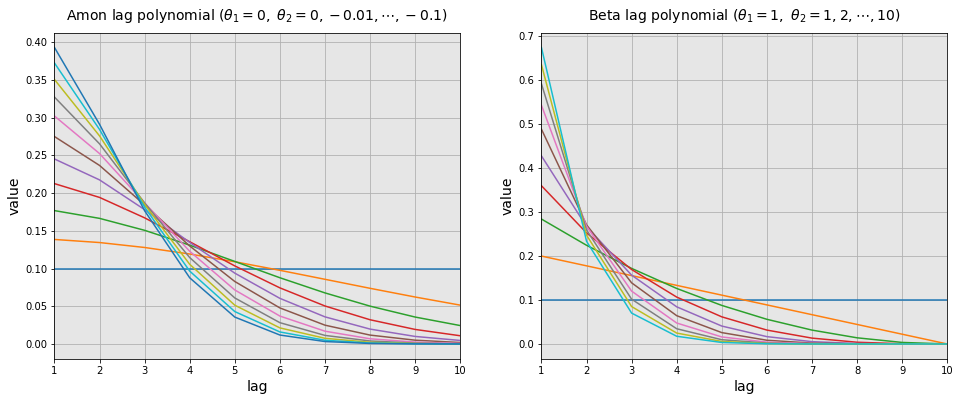
\includegraphics[scale=0.47]{images/lag_polynomials.png}
\caption{Amon and Beta lag polynomials for fixed $\theta_1$ values}
\label{fig_c3_s2_ss2_1}
\end{figure}

With this first simplification only $\theta_2$ remains to be estimated, which considerably simplifies the work of a numerical solver.

The second simplification is best understood by rewriting \ref{equation_c3_s2_ss1_2} in compact form as:

\begin{equation}
y = c + Y \gamma + \beta_1 \ X_1 \ w_1 + \cdots + \beta_n \ X_n \ w_n + \varepsilon
\label{equation_c3_s2_ss2_3}
\end{equation}

\newpage

with:

\begin{lflalign}
y = \left( \begin{matrix} y_{1} \\ y_{2} \\ \vdots \\ y_{T} \end{matrix} \right) \hspace{5mm}
c = \left( \begin{matrix} \mu \\ \mu \\ \vdots \\ \mu \end{matrix} \right) \hspace{5mm}
Y = \left( \begin{matrix} y_{0} & y_{-1} & \cdots & y_{-p} \\ y_{1} & y_{0} & \cdots & y_{-p-1} \\ \vdots & \vdots & \ddots & \vdots \\ y_{T-1} & y_{T-2} & \cdots & y_{T-p)} \end{matrix} \right) \hspace{5mm}
\gamma = \left( \begin{matrix} \gamma_1 \\ \gamma_2 \\ \vdots \\ \gamma_p \end{matrix} \right) \nonumber \\
X_i = \left( \begin{matrix} x_{i,m} & x_{i,m-1} & \cdots & x_{i,m-(q-1)} \\ x_{i,2m} & x_{i,2m-1} & \cdots & x_{i,2m-(q-1)} \\ \vdots & \vdots & \ddots & \vdots \\ x_{i,Tm} & x_{i,Tm-1} & \cdots & x_{i,Tm-(q-1)} \end{matrix} \right) \hspace{5mm}
w_i = \left( \begin{matrix} w_{i1} \\ w_{i2} \\ \vdots \\ w_{iq} \end{matrix} \right) \hspace{5mm}
\varepsilon = \left( \begin{matrix} \varepsilon_{1} \\ \varepsilon_{2} \\ \vdots \\ \varepsilon_{T} \end{matrix} \right)
\label{equation_c3_s2_ss2_4}
\end{lflalign}

Assume now that the weights $w_1, \cdots, w_n$ are known (i.e. the parameters $\theta_1, \cdots, \theta_n$ are known). Then defining the tranformed regressors $\tilde{X}_i = w_i X_i$, equation \ref{equation_c3_s2_ss2_3} can be reformulated as a standard linear regression:

\begin{equation}
y = X \delta + \varepsilon
\label{equation_c3_s2_ss2_5}
\end{equation}

with:

\begin{equation}
X = \left( \begin{matrix} 1 & Y & \tilde{X}_1 & \tilde{X}_2 & \cdots & \tilde{X}_n \end{matrix} \right) \hspace{10mm}
\delta = \left( \begin{matrix} c \\ \gamma \\ \beta_1 \\ \vdots \\ \beta_n \end{matrix} \right) \hspace{10mm}
\tilde{X}_i = X_i \ w_i
\label{equation_c3_s2_ss2_6}
\end{equation}

where $\delta$ is the vector of unknown coefficients that remain to be estimated. Assuming normality of the residuals as in \ref{equation_c3_s2_ss1_1}, the log likelihood of model \ref{equation_c3_s2_ss2_5} is proportional to:

\begin{equation}
\LL \propto - 0.5 \ (y - X \delta)' \ (y - X \delta)
\label{equation_c3_s2_ss2_7}
\end{equation}

This likelihood function is the so-called ``profile likelihood'' of \cite{Ghysels2016b}, owing its name to the fact that it is done conditional on $w_1, \cdots, w_n$. Maximizing \ref{equation_c3_s2_ss2_7} yields the standard OLS estimator:

\begin{equation}
\hat{\delta} = (X'X)^{-1} (X'y)
\label{equation_c3_s2_ss2_8}
\end{equation}

Substituting $\hat{\delta}$ back in the likelihood function \ref{equation_c3_s2_ss2_7} yields:

\begin{equation}
\LL_{\theta} \propto - 0.5 \ (y - X (X'X)^{-1} (X'y))' \ (y - X (X'X)^{-1} (X'y))
\label{equation_c3_s2_ss2_9}
\end{equation}

where the notation $\LL_{\theta}$ stresses the fact the likelihood \ref{equation_c3_s2_ss2_9} does not depend on $\delta$ anymore, but only on $\theta = \{ \theta_1, \cdots, \theta_n \}$ through $X$. It is then straightforward that the value of $\theta$ that maximizes \ref{equation_c3_s2_ss2_9} also maximizes the likelihood of the model, so that a maximum likelihood estimator of $\theta$ can obtain as:

\begin{equation}
\hat{\theta} =  \underset{\theta}{argmax} \left( - 0.5 \ (y - X (X'X)^{-1} (X'y))' \ (y - X (X'X)^{-1} (X'y)) \right)
\label{equation_c3_s2_ss2_10}
\end{equation}

which can simplify further into:

\begin{equation}
\hat{\theta} = \underset{\theta}{argmax} \left( y' X (X'X)^{-1} X' y \right)
\label{equation_c3_s2_ss2_11}
\end{equation}

\ref{equation_c3_s2_ss2_8} and \ref{equation_c3_s2_ss2_11} thus provide an efficient algorithm to estimate the MIDAS model:

\textbf{Algorithm 2: MIDAS regression} \vspace{3mm} \\
1. Use a numerical solver to find $\hat{\theta} = \underset{\theta}{argmax} \left( y' X (X'X)^{-1} X' y \right)$.

2. Once $\theta$ is known, calculate $X$, then compute $\hat{\delta} = (X'X)^{-1} (X'y)$.

The advantage of this approach compared to brute strength estimation of \ref{equation_c3_s2_ss2_2} is that the numerical part of the algorithm is here reduced to $\theta$ instead of all the parameters. The space on which the solver has to work is thus smaller, which increases the chance of success.


\subsection{Prediction}
\label{chapter3_section2_subsection3}


The MIDAS model is primarily intended for prediction purposes. Assume one wants to produce a one-step ahead prediction. This can be obtained by updating \ref{equation_c3_s2_ss1_2} by one period to obtain:

\begin{equation}
y_{t+1} = \mu + \sum_{j=1}^{p} \gamma_i \ y_{t+1-j} + \sum_{i=1}^{n} \beta_i \big( \sum_{j=1}^{q}  w_{ij} \  x_{i,(t+1)m+1-j} \big) + \varepsilon_{t+1}
\label{equation_c3_s2_ss3_1}
\end{equation}

\ref{equation_c3_s2_ss3_1} requires knowledge of the predictions $x_{i,t+1}, x_{i,t+2}, \cdots, x_{i,(t+1)m}$, which may be difficult or impossible to obtain. For this reason, \cite{Ghysels2016} proposes a more direct approach to forecasting in the context of MIDAS models. Define the $h$-step ahead MIDAS regression as:

\begin{equation}
y_{t+h} = \mu + \sum_{j=1}^{p} \gamma_i \ y_{t+1-j} + \sum_{i=1}^{n} \beta_i \big( \sum_{j=1}^{q}  w_{ij} \  x_{i,tm+1-j} \big) + \varepsilon_{t+h}
\label{equation_c3_s2_ss3_2}
\end{equation}

Taking expectations on both sides of \ref{equation_c3_s2_ss3_2}, a prediction $\hat{y}_{t+h}$ can easily be obtained from known feature values up to period $t$:

\begin{equation}
\hat{y}_{t+h} = \mu + \sum_{j=1}^{p} \gamma_i \ y_{t+1-j} + \sum_{i=1}^{n} \beta_i \big( \sum_{j=1}^{q}  w_{ij} \  x_{i,tm+1-j} \big)
\label{equation_c3_s2_ss3_3}
\end{equation}

With this method, the model becomes specific to the prediction $h$-steps ahead. In other words, one must now estimate a different model for each forecast horizon $h$.

Estimating the $h$-step ahead MIDAS regression is similar to the regular MIDAS model, except the matrices of regressors are now defined as:

\begin{equation}
Y = \left( \begin{matrix} y_{1-h} & y_{1-h-1} & \cdots & y_{1-h-(p-1)} \\ y_{2-h} & y_{2-h-1} & \cdots & y_{2-h-(p-1)} \\ \vdots & \vdots & \ddots & \vdots \\ y_{T-h} & y_{T-h-1} & \cdots & y_{T-h-(p-1)} \end{matrix} \right) \hspace{5mm}
X_i = \left( \begin{matrix} x_{i,m(1-h)} & x_{i,m(1-h)-1} & \cdots & x_{i,m(1-h)-(q-1)} \\ x_{i,m(2-h)} & x_{i,m(2-h)-1} & \cdots & x_{i,m(2-h)-(q-1)} \\ \vdots & \vdots & \ddots & \vdots \\ x_{i,m(T-h)} & x_{i,m(T-h)-1} & \cdots & x_{i,m(T-h)-(q-1)} \end{matrix} \right)
\label{equation_c3_s2_ss3_4}
\end{equation}



\subsection{Application}
\label{chapter3_section2_subsection4}


Besides forecasts, the MIDAS regression can also be used to assess the relative importance of each high frequency feature in predicting the low frequency variable, through examination of the lag structure. To do so, a one-step ahead MIDAS regression is estimated on the reduced macroeconomic dataset of the project. The benchmark used is $q=6$ high frequency lags, with a corresponding $p=2$ low frequency lags. 

Figure \ref{fig_c3_s2_ss4_1} reports the lag structure of the MIDAS model, for both the Almon and the Beta lag polynomial approaches. The features are normalised to avoid potential scale effects. 

\newpage

\begin{figure}[H]
\centering
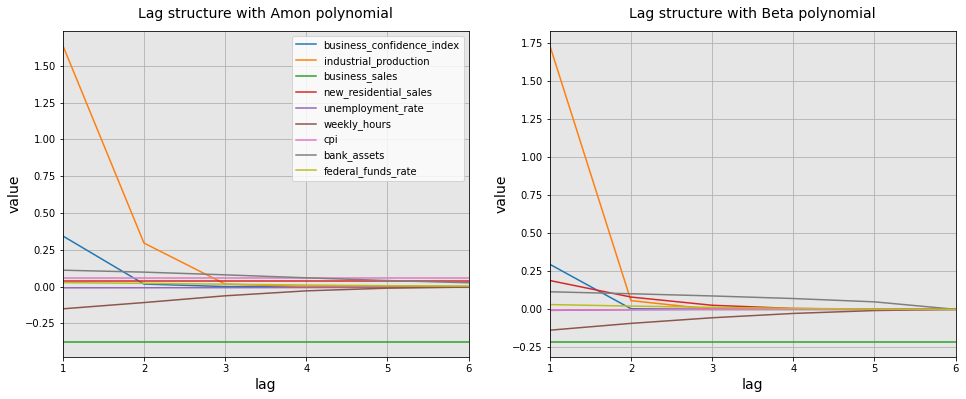
\includegraphics[scale=0.46]{images/lag_structure.png}
\caption{Amon and Beta lag polynomials for fixed $\theta_1$ values}
\label{fig_c3_s2_ss4_1}
\end{figure}

The two approaches yield fairly consistent estimates, with only small differences in magnitude observed. The main lesson from the plot is that over the 9 features included in the model, only 4 seem to have a strong predictive power on quarterly GDP: industrial production, the business confidence index, business sales, and weekly hours. The other variables contribute only marginally to GDP growth, and their lags are flat overall.

The strong positive correlations with industrial production and business confidence index makes sense, as the former is an important component of GDP, while the latter acts as a direct proxy. The negative correlation with business sales and weekly hours looks more surprising. However, the model considered is a one-step ahead MIDAS model. This may thus simply be the reflect that higher business sales and weekly hours today imply less production one quarter ahead, in an overshooting fashion.

\newpage

